
%(BEGIN_QUESTION)
% Copyright 2012, Tony R. Kuphaldt, released under the Creative Commons Attribution License (v 1.0)
% This means you may do almost anything with this work of mine, so long as you give me proper credit

This doorbell refuses to make any sound when the pushbutton is pressed.  An electrician begins to diagnose the problem, measuring 120 volts AC between the ``hot'' and ``neutral'' terminals on receptacle ``A'', and 0 volts AC between terminals {\bf L} and {\bf M} when the pushbutton is not being pressed.

$$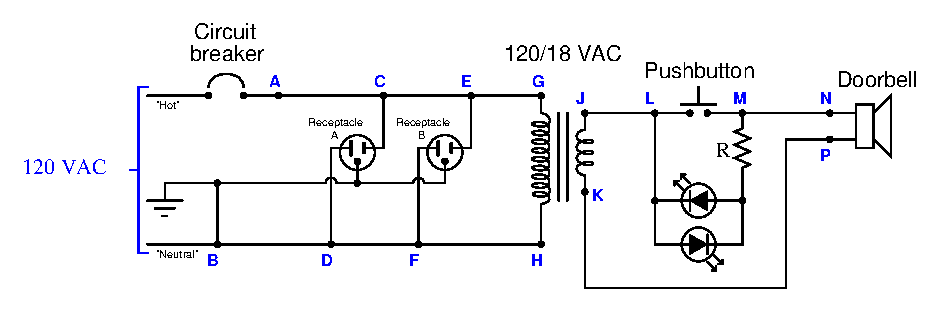
\includegraphics[width=15.5cm]{i01112x01.eps}$$

Identify the likelihood of each specified fault for this circuit.  Consider each fault one at a time (i.e. no coincidental faults), determining whether or not each fault could independently account for {\it all} measurements and symptoms in this circuit.

% No blank lines allowed between lines of an \halign structure!
% I use comments (%) instead, so that TeX doesn't choke.

$$\vbox{\offinterlineskip
\halign{\strut
\vrule \quad\hfil # \ \hfil & 
\vrule \quad\hfil # \ \hfil & 
\vrule \quad\hfil # \ \hfil \vrule \cr
\noalign{\hrule}
%
% First row
{\bf Fault} & {\bf Possible} & {\bf Impossible} \cr
%
\noalign{\hrule}
%
% Another row
Circuit breaker tripped &  &  \cr
%
\noalign{\hrule}
%
% Another row
Transformer primary winding failed open &  &  \cr
%
\noalign{\hrule}
%
% Another row
Transformer secondary winding failed open &  &  \cr
%
\noalign{\hrule}
%
% Another row
Resistor failed open &  &  \cr
%
\noalign{\hrule}
%
% Another row
Resistor failed shorted &  &  \cr
%
\noalign{\hrule}
%
% Another row
Open wire between K and P &  &  \cr
%
\noalign{\hrule}
%
% Another row
Doorbell unit failed open &  &  \cr
%
\noalign{\hrule}
%
% Another row
Doorbell unit failed shorted &  &  \cr
%
\noalign{\hrule}
} % End of \halign 
}$$ % End of \vbox


\underbar{file i01112}
%(END_QUESTION)





%(BEGIN_ANSWER)

% No blank lines allowed between lines of an \halign structure!
% I use comments (%) instead, so that TeX doesn't choke.

$$\vbox{\offinterlineskip
\halign{\strut
\vrule \quad\hfil # \ \hfil & 
\vrule \quad\hfil # \ \hfil & 
\vrule \quad\hfil # \ \hfil \vrule \cr
\noalign{\hrule}
%
% First row
{\bf Fault} & {\bf Possible} & {\bf Impossible} \cr
%
\noalign{\hrule}
%
% Another row
Circuit breaker tripped &  & $\surd$ \cr
%
\noalign{\hrule}
%
% Another row
Transformer primary winding failed open & $\surd$ &  \cr
%
\noalign{\hrule}
%
% Another row
Transformer secondary winding failed open & $\surd$ &  \cr
%
\noalign{\hrule}
%
% Another row
Resistor failed open &  & $\surd$ \cr
%
\noalign{\hrule}
%
% Another row
Resistor failed shorted &  & $\surd$ \cr
%
\noalign{\hrule}
%
% Another row
Open wire between K and P & $\surd$ &  \cr
%
\noalign{\hrule}
%
% Another row
Doorbell unit failed open & $\surd$ &  \cr
%
\noalign{\hrule}
%
% Another row
Doorbell unit failed shorted &  & $\surd$ \cr
%
\noalign{\hrule}
} % End of \halign 
}$$ % End of \vbox


%(END_ANSWER)





%(BEGIN_NOTES)

\filbreak \vskip 20pt \vbox{\hrule \hbox{\strut \vrule{} {\bf Virtual Troubleshooting} \vrule} \hrule}

\noindent
{\bf Predicting the effect of a given fault:} present each of the following faults to the students, one at a time, having them comment on all the effects each fault would produce.

\begin{itemize}
\item{} 
\item{} 
\item{} 
\end{itemize}


\vskip 10pt


\noindent
{\bf Identifying possible/impossible faults:} present symptoms to the students and then have them determine whether or not a series of suggested faults could account for all the symptoms, explaining {\it why} or {\it why not} for each proposed fault:

\begin{itemize}
\item{} Symptom: {\it }
\item{}  -- {\bf Yes/No}
\item{}  -- {\bf Yes/No}
\item{}  -- {\bf Yes/No}
\end{itemize}


\vskip 10pt


\noindent
{\bf Determining the utility of given diagnostic tests:} present symptoms to the students and then propose the following diagnostic tests one by one.  Students rate the value of each test, determining whether or not it would give useful information (i.e. tell us something we don't already know).  Students determine what different results for each test would indicate about the fault, if anything:

\begin{itemize}
\item{} Symptom: {\it }
\item{}  -- {\bf Yes/No}
\item{}  -- {\bf Yes/No}
\end{itemize}


\vskip 10pt


\noindent
{\bf Diagnosing a fault based on given symptoms:} imagine the secondary winding fails open in the transformer (don't reveal the fault to students!).  Present the operator's observation(s) to the students, have them consider possible faults and diagnostic strategies, and then tell them the results of tests they propose based on the following symptoms, until they have properly identified the nature and location of the fault:

\begin{itemize}
\item{} {\it Doorbell won't ring ; breaker isn't tripped}
\item{} $V_{CD}$ = 120 VAC
\item{} $V_{EF}$ = 120 VAC
\item{} $V_{GH}$ = 120 VAC
\item{} $V_{JK}$ = 0 VAC
\item{} $V_{LM}$ = 0 VAC (with switched pressed or released)
\item{} $V_{NP}$ = 0 VAC (with switched pressed or released)
\item{} $R_{GH}$ (with breaker off) = 75 $\Omega$
\item{} $R_{JK}$ (with breaker off) = 12.5 M$\Omega$
\end{itemize}

%INDEX% Electronics review: AC transformer circuit
%INDEX% Troubleshooting review: electric circuits

%(END_NOTES)


